\chapter{General Relativity and the fundamental observations of cosmology}

\section{General Relativity}

We have seen in the previous lecture how the incompatibility between Newtonian gravity and Special Relativity, in addition to the equivalence principle, leads us to the new picture of General Relativity (GR), in which the effects of gravity are described by the curvature of spacetime. As we learned in lecture 2, all the geometrical properties of a space (or a spacetime in the case of GR) are encoded in the metric tensor, so it is natural to regard the metric as the gravitational field that affects the motion of particles. It remains to understand how do we calculate the metric in the first place. This will be the subject of this section.

\subsection{The motion of particles and geodesics}

Let us begin by summarizing what we learned in the previous lecture about the relation between the motion of particles and the metric of spacetime. Given two events with spacetime coordinates $(x^0,x^1,x^2,x^3)$ and $(x^0+dx^0,x^1+dx^1,x^2+dx^2,x^3+dx^3)$,\footnote{In chapter 2 we defined $x^0=ct$, $x^1=x$, $x^2=y$, $x^3=z$. Here we will abandon this convention; the coordinates $x^{\mu}$ now refer to an arbitrary coordinate system. For example, in spherical coordinates (see chapter 3) we would have $x^0=ct$, $x^1=r$, $x^2=\theta$, $x^3=\phi$. (We will always consider coordinate systems in which $x^0$ is a time coordinate and $x^1$, $x^2$, $x^3$ are spatial coordinates; however, there are examples of coordinate systems in which this not the case.)} the spacetime interval $ds$ between them is given by
\begin{equation} \label{eq:line_element}
ds^2=g_{\mu\nu}dx^{\mu}dx^{\nu}.
\end{equation}
Remember that in GR the metric is a function of spacetime, i.e.\ $g_{\mu\nu}=g_{\mu\nu}(x^0,x^1,x^2,x^3)$. It is only in SR (that is, in the absence of gravity) that we can find coordinates where $g_{\mu\nu}$ is constant everywhere. We can consider these two events to be related to a particle located at position $(x^1,x^2,x^3)$ at time $x^0$, and then located at $(x^1+dx^1,x^2+dx^2,x^3+dx^3)$ at time $x^0+dx^0$. This is simply a way of keeping track of the particle's motion by means of successive, infinitesimally close events.

Recall that for a particle we have $ds^2<0$. This is easy to see in SR, where we can choose a Cartesian coordinate system $(ct,x,y,z)$ in which $g_{\mu\nu}=\eta_{\mu\nu}$. If we assume that the particle is moving in the $x$-direction, so that $dy=0$ and $dz=0$, then eq.\ (\ref{eq:line_element}) becomes
\begin{equation}
\begin{split}
ds^2&=-c^2dt^2+dx^2\\
&=-dt^2\left(c^2-\left(\frac{dx}{dt}\right)^2\right)\\
&=-dt^2\left(c^2-v^2\right),
\end{split}
\end{equation}
where $v=dx/dt$ is the velocity of the particle. Since the particle cannot move faster than light, we must have that $(c^2-v^2)>0$, and therefore $ds^2<0$. Having shown that $ds^2<0$ in SR, we can immediately conclude that $ds^2<0$ also in GR. This follows from the fact that at any point in a curved spacetime we can choose coordinates where, in a small neighborhood around the point, the metric is $g_{\mu\nu}\approx\eta_{\mu\nu}$.

The {\it proper time} $d\tau$ elapsed along a particle's trajectory is defined as
\begin{equation} \label{eq:proper_time_dtau}
d\tau=\sqrt{-\frac{ds^2}{c^2}}=\frac{1}{c}\sqrt{-g_{\mu\nu}dx^{\mu}dx^{\nu}}.
\end{equation}
Notice that the expression inside the square root is positive since $ds^2<0$ for a particle, and therefore $d\tau$ is a positive real quantity. The above definition holds for an infinitesimal path, but we can find the proper time elapsed along a finite trajectory by integrating $d\tau$ along the path traveled by the particle. Thus, if a particle moves from some spacetime point $A$ to some other spacetime point $B$, then the proper time along the path is given by
\begin{equation}
\begin{split}
\Delta\tau(A\to B)&=\int_A^B d\tau\\
&=\frac{1}{c}\int_A^B \sqrt{-g_{\mu\nu}dx^{\mu}dx^{\nu}}.\\
\end{split}
\end{equation}
Physically, the proper time corresponds to the time measured by a clock moving together with the particle. Notice that, although the spacetime interval along a particle's path cannot be measured using rulers, it can be measured using a clock.

Given the trajectory that a particle travels we now know how to compute the proper time elapsed from the initial point $A$ to the final point $B$ of the path. But suppose we are given nothing but the spacetime coordinates of the points $A$ and $B$, and we are asked to find the path that a particle takes when going from $A$ to $B$. Among all the possible paths the particle can take between $A$ and $B$, the actual path will be the one that {\it maximizes} the elapsed proper time $\Delta\tau(A\to B)$. With this prescription, we can in principle predict the motion of particles from the knowledge of the metric of the spacetime.

From a geometrical point of view, the trajectories that maximize the proper time between two given points are called {\it geodesics} of the spacetime. Geodesics are easy to visualize in 2-dimensional spaces; in this case we do not have to deal with proper time (there is no time dimension) and $ds$ is the usual length we would measure with a ruler. Thus, given two points $A$ and $B$, the length of a path connecting them is simply
\begin{equation}
\Delta s(A\to B)=\int_A^B ds.
\end{equation}
The geodesic is then given by the path that {\it minimizes} $\Delta s(A\to B)$.\footnote{Notice that in spacetimes geodesics are the paths that maximize the proper time, whereas in spaces (no time dimension) geodesics are the paths that minimize the length. The reason for this difference has to do with the fact that $ds^2$ is not necessarily positive in spacetimes.} Fig.\ \ref{fig:lec4_1} shows two examples of 2-dimensional spaces, the flat plane and the sphere. Clearly, the geodesics on the plane correspond to straight lines; any other curve joining two given points will obviously have a larger length. Perhaps less obvious is that the geodesics on the sphere correspond to circular segments around the center of the sphere. For example, if point $A$ is the north pole of the sphere and $B$ is a point on the equator, then the geodesic connecting $A$ and $B$ goes along ``meridian'' through these points.
\begin{figure}[ht]
\begin{center}
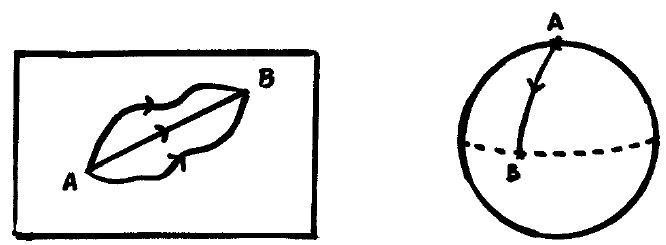
\includegraphics[scale=0.5]{Draw/lec4_1.png}
\end{center}
\caption{Geodesics in 2-dimensional spaces}
\label{fig:lec4_1}
\end{figure}

One final quantity that we need to define, which we will need later, is the {\it 4-velocity} of a particle. Since the proper time $\tau$ is a quantity that increases monotonically along a particle's trajectory, we can use it to parametrize the path traveled by the particle. In other words, we can think of the spacetime coordinates $x^{\mu}$ of the particle as being functions of $\tau$, i.e.\ $x^{\mu}(\tau)$. The 4-velocity of the particle is then defined as
\begin{equation}
U^{\mu}\equiv \frac{dx^{\mu}}{d\tau}.
\end{equation}
Of course, the coordinates $x^{\mu}$ refer to a specific coordinate system, and therefore $U^{\mu}$ will depend on the specific coordinate system or reference frame we are using. As an example, consider a reference frame where a particle is at rest. Since the particle is not moving in space, we have that $x^1$, $x^2$ and $x^3$ are constants, and therefore $U^i=dx^i/d\tau=0$.\footnote{Recall that greek indices range from 0 to 3, whereas latin indices range from 1 to 3.} On the other hand, the time coordinate $x^0$ is equal to $c\tau$, since by definition $\tau$ is the time measured in the frame where the particle is at rest. Therefore $U^0=dx^0/d\tau=d(c\tau)/d\tau=c$. In summary, the 4-velocity vector of a particle at rest is given by $(c,0,0,0)$.

A useful property of the 4-velocity that we will use later is that it is {\it normalized}. What this means is simply that $g_{\mu\nu}U^{\mu}U^{\nu}$ has a constant value which turns out to be $-c^2$. Indeed, using the definition of $U^{\mu}$ and eq.\ (\ref{eq:proper_time_dtau}), we have
\begin{equation}
\begin{split}
g_{\mu\nu}U^{\mu}U^{\nu}&=g_{\mu\nu}\frac{dx^{\mu}}{d\tau}\frac{dx^{\nu}}{d\tau}\\
&=\frac{g_{\mu\nu}dx^{\mu}dx^{\nu}}{d\tau^2}\\
&=\frac{ds^2}{-ds^2/c^2}=-c^2
\end{split}
\end{equation}
\begin{equation}
\Rightarrow~~~~g_{\mu\nu}U^{\mu}U^{\nu}=-c^2.
\end{equation}


\subsection{The Einstein equations}

We know how to calculate the motion of particles in spacetime if we know the metric. But how do we find the metric in the first place? In principle we could measure the metric by observing how particles move, but unless we do such observations on all points in space at all times (which is obviously impractical), we will never know what the metric is everywhere in the spacetime. Instead, we would like to be able to calculate the metric starting from the knowledge of the sources of the gravitational field. For example, in Newtonian physics, just by knowing the mass of the Sun we can find the (approximate) gravitational field in the whole solar system, thanks to Newton's law of gravitation.

The analog of Newton's law in GR is given by the {\it Einstein equations}:
\begin{equation} \label{eq:einstein_eqs}
G^{\mu\nu}=\frac{8\pi G}{c^4}T^{\mu\nu},
\end{equation}
where $G$ is Newton's constant (the same that appears in Newton's law), $c$ is the speed of light, $G^{\mu\nu}$ is the {\it Einstein tensor}, and $T^{\mu\nu}$ is the {\it energy-momentum tensor}. The Einstein tensor is quite complicated and so we will not give its precise definition. The only thing you need to know about it is that it depends solely on the metric (and on first and second derivatives of the metric) through the Riemann tensor (see chapter 3), which means that $G^{\mu\nu}=0$ when the spacetime is flat, since the Riemann tensor vanishes everywhere in Minkowski spacetime.

The energy-momentum tensor (also known as the stress-energy tensor), as it name suggests, depends on the energy and momentum of the sources present in the spacetime (and also possibly on the metric). There is no general explicit formula for $T^{\mu\nu}$, since it will depend on what kind of sources we are dealing with; in the next section we will see an example relevant to cosmology. We remarked in chapter 2 that in relativity energy and momentum should not be considered as independent entities, since energy can be transformed into momentum, and vice versa, by means of a Lorentz transformation. It should not be surprising then that it is both the energy {\it and} the momentum of the sources what gives rise to a gravitational field. This is in marked contrast to what happens in Newtonian gravity, where only the mass (which, as you know, is a form of energy) is relevant in the gravitational interaction.

Both $G^{\mu\nu}$ and $T^{\mu\nu}$ are symmetric tensors, which means that
\begin{equation}
G^{\mu\nu}=G^{\nu\mu},\mbox{ and }~~T^{\mu\nu}=T^{\nu\mu}.
\end{equation}
This implies that, although there are 16 possible combinations for the indices $\mu\nu$, the Einstein equations are really 10 independent equations. This correctly matches the number of independent components of the metric $g_{\mu\nu}$, which you may remember is also a symmetric tensor.

\par\vspace{\baselineskip}

{\bf Exercise.} Show that a symmetric $4\times4$ matrix has 10 independent components.

\par\vspace{\baselineskip}

\section{Perfect fluids}

A fluid is a continuous substance that can be deformed under the application of a force or stress. A fluid has no fixed shape, and will tend to assume the shape of its container. Fig.\ \ref{fig:lec4_2} shows a volume of fluid in which several {\it fluid elements} have been drawn. A fluid element is a portion of the fluid that is macroscopically small, meaning that we can approximate it as being homogeneous, but microscopically large, meaning that it contains a very large number of particles so that a fluid description is appropriate. The fact that a fluid element is homogeneous implies that it can be characterized by its density $\rho$ (mass per unit volume), its pressure $p$ (force per unit area exerted perpendicularly on its neighbors), its shear viscosity $f_s$ (the antislipping force; see fig.\ \ref{fig:lec4_2}), and its 4-velocity $U^{\mu}$. A {\it perfect fluid} is one where $f_s=0$ for all fluid elements. It turns out that many sources of energy in astrophysics and cosmology can be well approximated 
as perfect fluids, and so we will focus on them in the following discussion.
\begin{figure}[ht]
\begin{center}
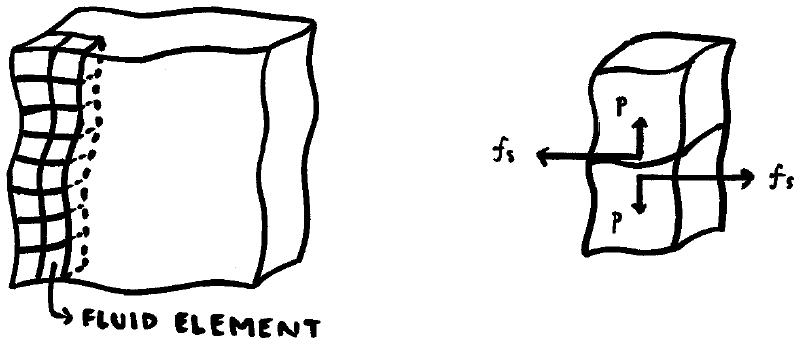
\includegraphics[scale=0.5]{Draw/lec4_2.png}
\end{center}
\caption{Perfect fluids}
\label{fig:lec4_2}
\end{figure}

After defining the properties of individual fluid elements, we can extend these definitions to the whole fluid. We will characterize a fluid by the three functions $\rho(t,x,y,z)$, $p(t,x,y,z)$, and $U^{\mu}(t,x,y,z)$, which are defined as:\footnote{Here we are using the familiar Cartesian coordinates $(t,x,y,z)$ just to make the discussion simpler, but note that all these definitions can be applied in an arbitrary reference frame with coordinates $(x^0,x^1,x^2,x^3)$.}
\begin{itemize}
\item $\rho(t,x,y,z)$ is the density of the fluid element located at the position $(x,y,z)$ at the time $t$.
\item $p(t,x,y,z)$ is the pressure of the fluid element located at the position $(x,y,z)$ at the time $t$.
\item $U^{\mu}(t,x,y,z)$ is the 4-velocity of the fluid element located at the position $(x,y,z)$ at the time $t$.
\end{itemize}
With these definitions we can now write down the energy-momentum tensor of a perfect fluid:
\begin{equation} \label{eq:perfect_fluid_tmunu}
T^{\mu\nu}=\left(\rho+\frac{p}{c}\right)U^{\mu}U^{\nu}+pcg^{\mu\nu}.
\end{equation}
Here the tensor $g^{\mu\nu}$ corresponds, by definition, to the components of the {\it matrix inverse} of $g$. Recall that, given a matrix $M$, its inverse matrix is defined as the matrix $M^{-1}$ such that $MM^{-1}=I$ (where $I$ is the identity matrix). As an example, consider the Minkowski metric,
\begin{equation}
\eta=\left( \begin{array}{cccc} -1 & 0 & 0 & 0 \\ 
0 & 1 & 0 & 0 \\
0 & 0 & 1 & 0 \\
0 & 0 & 0 & 1\end{array} \right).
\end{equation}
Its inverse matrix is given by
\begin{equation}
\eta^{-1}=\left( \begin{array}{cccc} -1 & 0 & 0 & 0 \\ 
0 & 1 & 0 & 0 \\
0 & 0 & 1 & 0 \\
0 & 0 & 0 & 1\end{array} \right).
\end{equation}
We leave as an excercise for you to check that
\begin{equation}
\eta\eta^{-1}=\left( \begin{array}{cccc} 1 & 0 & 0 & 0 \\ 
0 & 1 & 0 & 0 \\
0 & 0 & 1 & 0 \\
0 & 0 & 0 & 1\end{array} \right)=I.
\end{equation}
In this example we have that $\eta^{-1}=\eta$. However, note that this will not be true for a general metric $g$. That is why we need to distinguish $g_{\mu\nu}$ (the components of the metric $g$) from $g^{\mu\nu}$ (the components of the inverse metric $g^{-1}$).

\par\vspace{\baselineskip}

{\bf Exercise.} Consider the metric given by
\begin{equation}
ds^2=-c^2dt^2+Adx^2+Bdy^2+Cdz^2,
\end{equation}
where $A$, $B$, and $C$ are positive constants, and the coordinate system is $(ct,x,y,z)$.
\begin{itemize}
\item [(a)] Show that the components $g_{\mu\nu}$ of the metric are given by
\begin{equation}
g_{00}=-1,~~~~g_{11}=A,~~~~g_{22}=B,~~~~g_{33}=C,
\end{equation}
with all other components equal to zero.
\item [(b)] Write the metric in matrix form as
\begin{equation}
g=\left( \begin{array}{cccc} -1 & 0 & 0 & 0 \\ 
0 & A & 0 & 0 \\
0 & 0 & B & 0 \\
0 & 0 & 0 & C\end{array} \right),
\end{equation}
and from this find the inverse metric $g^{-1}$. Show that the components $g^{\mu\nu}$ of $g^{-1}$ are given by
\begin{equation}
g^{00}=-1,~~~~g^{11}=\frac{1}{A},~~~~g^{22}=\frac{1}{B},~~~~g^{33}=\frac{1}{C},
\end{equation}
with all other components equal to zero. Note that $g^{-1}\neq g$ in this example.
\end{itemize}

\par\vspace{\baselineskip}

Given a perfect fluid with some specified density $\rho(t,x,y,z)$, pressure $p(t,x,y,z)$, and 4-velocity $U^{\mu}(t,x,y,z)$, we could compute the energy-momentum tensor $T^{\mu\nu}$ from eq.\ (\ref{eq:perfect_fluid_tmunu}), plug the result in the Einstein equations (\ref{eq:einstein_eqs}), and solve for the metric $g_{\mu\nu}$ (in practice this can be very difficult though). As an example, let us find $T^{\mu\nu}$ for a perfect fluid at rest in Minkowski spacetime (i.e.\ $g_{\mu\nu}=\eta_{\mu\nu}$). Since the fluid is at rest, we have that the components of the 4-velocity are $U^0=c$ and $U^i=0$. Then we find
\begin{equation}
\begin{split}
T^{00}&=\left(\rho+\frac{p}{c}\right)U^{0}U^{0}+pc\eta^{00}\\
&=\left(\rho+\frac{p}{c}\right)c^2-pc=\rho c^2,
\end{split}
\end{equation}
and
\begin{equation}
T^{11}=pc\eta^{11}=pc,~~~~T^{22}=pc\eta^{22}=pc,~~~~T^{33}=pc\eta^{33}=pc.
\end{equation}
You can easily check that all other components of $T^{\mu\nu}$ vanish. Therefore we can write, in matrix form,
\begin{equation}
T^{\mu\nu}=\left( \begin{array}{cccc} \rho c^2 & 0 & 0 & 0 \\ 
0 & pc & 0 & 0 \\
0 & 0 & pc & 0 \\
0 & 0 & 0 & pc\end{array} \right).
\end{equation}


\section{Cosmology: Fundamental observations}

We are now ready to begin our study of cosmology. In this section we will cover the fundamental observational facts about the universe. We will see how these facts can be explained by the Big Bang model, in which the universe was born from an initial singularity and has been expanding ever since. These observations will also guide us in the task of modeling the universe mathematically in the framework of GR.

\subsection{The Olbers paradox}

Why is the night sky dark? This simple question summarizes what is known as the Olbers paradox. The paradox arises when we think of the universe as being static, infinitely old, infinitely large, and with an infinite number of stars. If we lived in such a universe, then in every direction we looked at in the night sky we should encounter a star along the line of sight, simply because there are infinitely many stars. The night sky should therefore be completely bright!

Let us look at this argument more closely. One could argue that our conclusion is incorrect because distant stars appear dimmer, and so they may not be visible in the night sky. Thus, if in one direction in the sky there were no nearby stars, then the night sky would be dark in that direction. This objection is wrong, however, because although the apparent brightness of stars decreases with distance, the number of stars along a given line of sight increases. This is illustrated in fig.\ \ref{fig:lec4_3}. Here $A$ and $B$ denote two directions in the sky; in direction $A$ we can see some nearby stars, which appear bright, whereas in direction $B$ we do not see nearby stars, but only dimmer stars that are farther away. Does the sky appear brighter in direction $A$ than in direction $B$? No, because in direction $B$ we also see more stars than in direction $A$. This is because our telescope collects light from a larger area in the sky as it observes at larger distances. This area is proportional to the square 
of the distance (since the area of a sphere is proportional to the radius squared), whereas the apparent brightness is inversely proportional to the distance squared.\footnote{To understant why the apparent brightness of a light source is proportional to the inverse squared distance, note that the energy per unit time (or luminosity) crossing a spherical surface of radius $R$ centered on the source is independent of $R$, since all the energy emitted by the source in some time interval must eventually reach the surface (assuming nothing absorbs the energy along the way). However, the energy flux (energy per unit time per unit area) is obtained by dividing the luminosity by the area of the surface, which is proportional to $R^2$.} Therefore the sky in direction $B$ appears as bright (on average) as in direction $A$.
\begin{figure}[ht]
\begin{center}
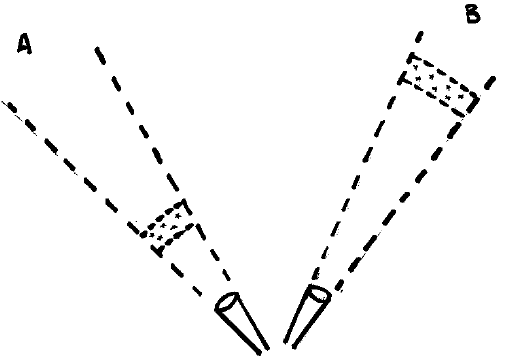
\includegraphics[scale=0.5]{Draw/lec4_3.png}
\end{center}
\caption{The Olbers paradox}
\label{fig:lec4_3}
\end{figure}

The paradox forces us to conclude that this model of the universe (static, infinitely old, infinitely large) must be incorrect. The universe is neither static nor infinitely old, but has some finite age and it is actually expanding, as predicted by the Big Bang model. The fact that the universe has a finite age immediately solves the Olbers paradox: even though the universe might be infinite in space and filled with an infinite number of stars, the light from very distant stars has not had enough time to reach us yet.

\subsection{The cosmological principle: the universe is homogeneous and isotropic}

On very large distance scales, larger than of order $100$ Mpc,\footnote{Recall that $1~{\rm pc}=3.3~{\rm ly}=3.1\times10^{16}$ m. Also, $1~{\rm Mpc}=10^6$ pc.} the universe is observed to be homogeneous and isotropic. This is the cosmological principle, which is essentially the statement that there are no special points in the universe. To be precise, homogeneous and isotropic spaces are defined as follows:
\begin{itemize}
\item {\bf Homogeneous space:} A space with no preferred locations; all points are equivalent.
\item {\bf Isotropic space:} A space where, around one or more points, there are no preferred directions; things look the same in every direction.
\end{itemize}
Notice that isotropy refers to a specific point in a space. For example, a cone is isotropic about the point at its vertex, but not about any other point (fig.\ \ref{fig:lec2_4}). The cone is actually an example of a space that is isotropic but not homogeneous, since clearly the vertex is a special point.\footnote{Notice that the space we are referring to is the 2-dimensional surface of the cone. We can of course visualize the cone as embedded in our 3-dimensional Euclidean space, but the properties of homogeneity and isotropy refer to the 2-dimensional surface in this example (as well as in the examples of the plane and the cylinder discussed next), and are completely independent on how the surface looks as viewed from outside.} The 2-dimensional surface of an infinite cylinder provides an example of a space that is homogeneous (since all points are equivalent) but not isotropic (since a person living in this 2-dimensional space would conclude that not all directions are equivalent; if he walked in the 
direction perpendicular to the axis of the cylinder he would return to the place where he started after some time, whereas this would not be true if he walked in the direction parallel to the axis).
\begin{figure}[ht]
\begin{center}
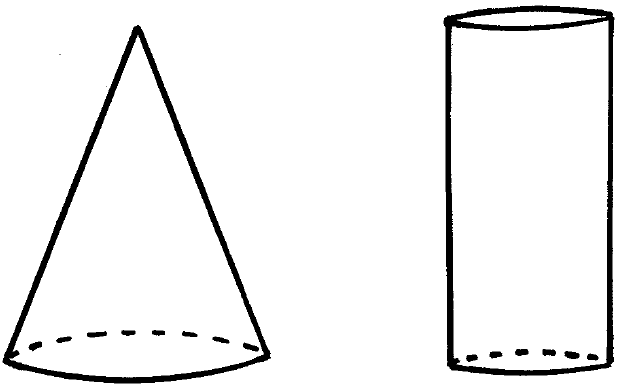
\includegraphics[scale=0.4]{Draw/lec4_4.png}
\end{center}
\caption{Homogeneous and isotropic spaces}
\label{fig:lec4_4}
\end{figure}

From the above examples we see that homogeneity and isotropy are really different concepts. However, if a space is isotropic around not just a few points but around {\it every} point, then it must also be homogeneous (if everything looks the same everywhere, then everywhere is the same). Spaces that are both homogeneous and isotropic are called {\it maximally symmetric spaces}. Examples of maximally symmetric spaces in 2 dimensions are the infinite flat plane and the surface of a sphere. Can you think of other examples? There is in fact one more maximally symmetric space, called the 2-dimensional hyperbolic space, which cannot be visualized (it cannot be embedded in our 3-dimensional Euclidean space, unlike the sphere). It turns out that this is true for any number of spatial dimensions. In 3 dimensions, for instance, the flat space (Euclidean space), the 3-sphere (the 3-dimensional analog of the the usual sphere), and the 3-dimensional hyperbolic space are the only examples of maximally symmetric spaces.\
footnote{The fact that there are exactly three examples of maximally symmetric spaces for any number of dimensions is actually true even if one of the dimensions is a time dimension. This will not be important for us, however. When we say that the universe is homogeneous and isotropic we are talking about the 3-dimensional space, without including the time dimension.} This fact will be important when we go to the task of writing down the possible metrics that can in principle describe our universe.

Returning to the cosmological principle, it is important to emphasize that the principle holds only for large scales. The universe is obviously neither homogeneous nor isotropic on small scales. For example, in the solar system clearly the position of the Sun is a special point, so there is no homogeneity. Also, the solar system has no isotropy, not even around the Sun, since clearly the direction parallel to the plane where the planets move is different from the direction perpendicular to it. It is only when we get to distance scales of order 100 Mpc that the universe begins to look homogeneous and isotropic. Fig.\ \ref{fig:lec4_5} shows an image of the universe as seen from the Earth containing over 2 million galaxies. Make an imaginary square with sides measuring about a tenth of the length of the image; the size of this square is a few hundred megaparsecs. You can see that as you move the square around the image, the number of galaxies contained inside is roughly the same no matter where you locate the 
square. This means that, on the scale of your square, the universe is homogeneous. Also, the galaxies contained inside the square, at any location, clearly do not distribute themselves with some preferred direction, meaning that on this scale the universe is also isotropic.
\begin{figure}[ht]
\begin{center}
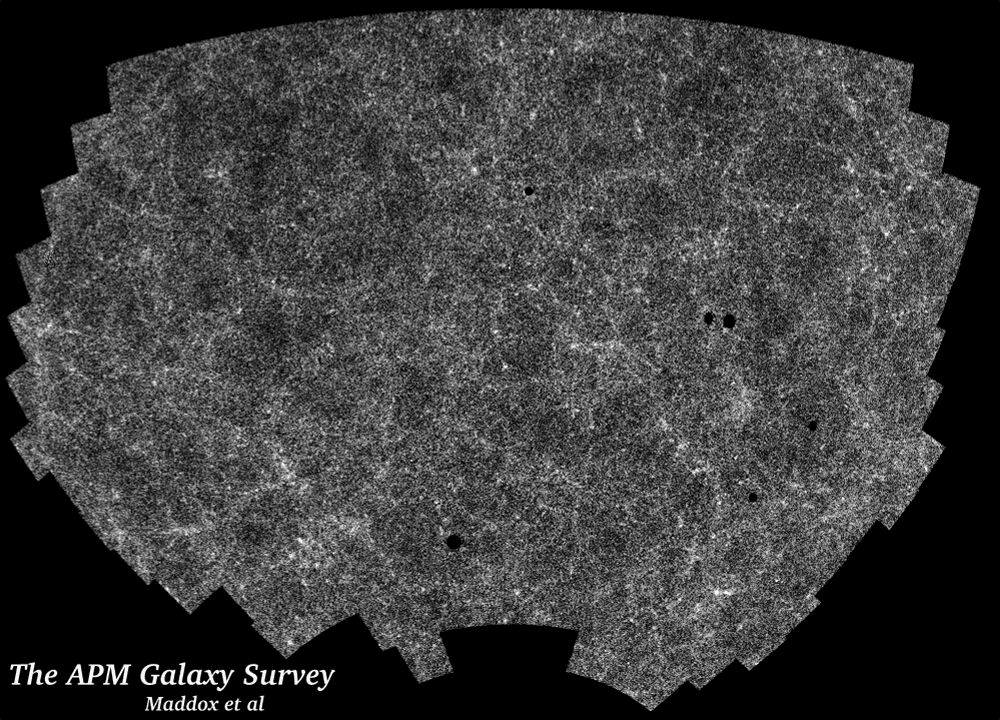
\includegraphics[scale=0.4]{Draw/lec4_5.png}
\end{center}
\caption{The APM Galaxy Survey (Image credit: Maddox et al., The University of Nottingham)}
\label{fig:lec4_5}
\end{figure}

\subsection{The universe is expanding}

In 1929 Edwin Hubble made one of the most extraordinary discoveries in the history of physics: the universe is expanding. This observational fact was the main motivation for the introduction of the Big Bang model, which provides the currently accepted theory of the evolution of the universe. It is fair to say, then, that Hubble's discovery marks the birth of modern cosmology.

Before going into a precise description of Hubble's observation, what is known as Hubble's law, we first need to introduce the concept of redshift in waves and explain the relativistic Doppler effect.

\subsubsection{Waves}

A wave is an oscillatory disturbance that transfers energy and momentum from one point to another, often without transferring particles or mass. Familiar examples include water waves, sound waves, and the waves on a string. These are all examples of {\it mechanical waves}, which are defined as waves that propagate through a medium whose material is deformed by the wave. Other types of waves include electromagnetic waves, gravitational waves, and quantum mechanical matter waves.

Waves can be characterized by their wavelength, frequency, and propagation speed. The wavelength $\lambda$ is given by the distance between two successive crests. Then, if $v$ is the speed of propagation (which depends on both the type of wave and the medium\footnote{The speed of propagation can also depend on the wavelength, in which case the wave is said to be dispersive. Water waves give an example of dispersive waves. We will be mainly interested in electromagnetic waves traveling in vacuum, which are not dispersive; in this case the speed of propagation is always $c$, regardless of the value of $\lambda$.}), the frequency is given by
\begin{equation}
f=\frac{v}{\lambda}.
\end{equation}
The frequency is a measure of the number of oscillations per unit time in a given point on the wave, and it is directly related to the energy transferred by the wave. Thus higher frequency means higher energy, and also longer wavelength. Fig.\ ?? shows the electromagnetic spectrum, the spectrum containing all different types of electromagnetic waves, from the most energetic ones (gamma rays) to the less energetic ones (radio waves). You can see that visible light, the only electromagnetic wave that the human eye can directly observe, constitutes only a small part of the complete spectrum.
\begin{figure}[ht]
\begin{center}
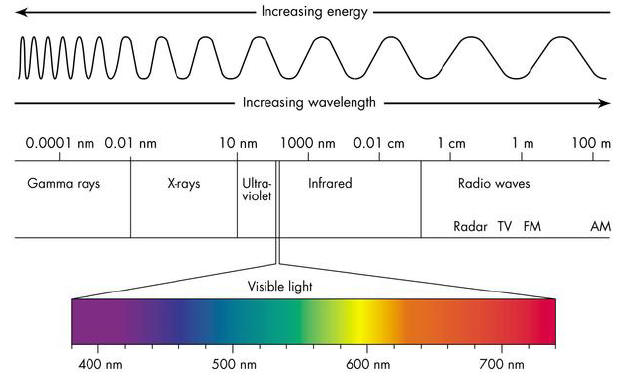
\includegraphics[scale=2]{Draw/lec4_6.png}
\end{center}
\caption{The electromagnetic spectrum (Source: \url{http://www.scimad.com})}
\label{fig:lec4_6}
\end{figure}

\subsubsection{Relativistic Doppler effect}

You may be already familiar with the usual nonrelativistic Doppler effect. This effect is essentially the statement that the wavelength of a wave changes if the observer is in motion relative to the source. In other words, the wavelength (and hence the frequency) of a wave depends on the reference frame. We will consider the particular case in which the source emitting an electromagnetic wave (say a light ray) is moving directly away from the observer with velocity $v$ (see fig.\ \ref{fig:lec4_7}).
\begin{figure}[ht]
\begin{center}
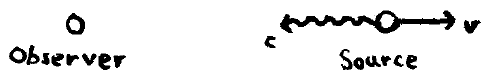
\includegraphics[scale=0.6]{Draw/lec4_7.png}
\end{center}
\caption{Relativistic Doppler effect}
\label{fig:lec4_7}
\end{figure}

In the reference frame of the source, the observer is moving away with speed $v$. The time $\Delta t_{\rm em}$ elapsed between the arrival of two successive wave crests equals the distance between the crests (which is $\lambda_{\rm em}$, the wavelength of the emitted wave) divided by relative velocity between the wave and the observer. That is
\begin{equation}
\Delta t_{\rm em}=\frac{\lambda_{\rm em}}{c-v}.
\end{equation}
In the reference frame of the observer this time is shorter due to the relativistic time dilation; see eq.\ (\ref{eq:time_dilation}). The observer actually measures
\begin{equation}
\Delta t_{\rm obs}=\Delta t_{\rm em}\sqrt{1-\frac{v^2}{c^2}}.
\end{equation}
Now, the observer measures the light ray to have a speed $c$, by the second postulate of SR. Therefore the wavelength measured by the observer is
\begin{equation}
\begin{split}
\lambda_{\rm obs}&=c\Delta t_{\rm obs}\\
&=c\Delta t_{\rm em}\sqrt{1-\frac{v^2}{c^2}}\\
&=\frac{c}{c-v}\sqrt{1-\frac{v^2}{c^2}}~\lambda_{\rm em}.
\end{split}
\end{equation}
Rearranging this equation we obtain
\begin{equation}
\begin{split}
\frac{\lambda_{\rm obs}}{\lambda_{\rm em}}&=\frac{\sqrt{1-\frac{v^2}{c^2}}}{\left(1-\frac{v}{c}\right)}\\
&=\frac{\sqrt{\left(1+\frac{v}{c}\right)\left(1-\frac{v}{c}\right)}}{\left(1-\frac{v}{c}\right)}\\
\end{split}
\end{equation}
\begin{equation}
\Rightarrow~~~~~~\frac{\lambda_{\rm obs}}{\lambda_{\rm em}}= \sqrt{\frac{1+\frac{v}{c}}{1-\frac{v}{c}}}.
\end{equation}
This is the expression of the relativistic Doppler effect for the case in which the source and the observer are moving away from each other. Notice that the right hand side is larger than 1, meaning that $\lambda_{\rm obs}>\lambda_{\rm em}$. This means that, to the observer, the source (a galaxy for instance) looks as if it were emitting light with larger wavelength than it actually is. The source looks ``more red'' to the observer. We say in this case that the light from the source is {\it redshifted}. Quantitatively, the redshift $z$ of the source is defined as
\begin{equation}
z=\frac{\lambda_{\rm obs}-\lambda_{\rm em}}{\lambda_{\rm em}}.
\end{equation}
Notice that by measuring the redshift of an object we can deduce the velocity at which it is receding from us. If the velocity of the object is small compared to the speed of light, so that $v/c\ll1$, we can approximate
\begin{equation}
\sqrt{\frac{1+\frac{v}{c}}{1-\frac{v}{c}}}\approx 1+\frac{v}{c}.
\end{equation}
Then the redshift will be approximately given by
\begin{equation}
z=\frac{\lambda_{\rm obs}}{\lambda_{\rm em}}-1\approx \frac{v}{c}.
\end{equation}
The relation between redshift and velocity is thus very simple in the nonrelativistic case; if we know $z$, then $v\approx cz$.

\par\vspace{\baselineskip}

{\bf Exercise.} Show that, in the general case (i.e.\ without assuming $v\ll c$), the velocity in terms of the redshift is given by the formula
\begin{equation}
\frac{v}{c}=\frac{(z+1)^2-1}{(z+1)^2+1}.
\end{equation}

\par\vspace{\baselineskip}

\subsubsection{Hubble's law}

Hubble's observation that the universe is expanding was based on the independent measurements of the redshift and distance of several nearby galaxies. What he found is that the redshift of a galaxy is directly proportional to its distance, a relation known as Hubble's law:
\begin{equation}
z=\frac{H_0}{c}d.
\end{equation}
In this equation $d$ is the distance to the galaxy, $c$ is the speed of light, and $H_0$ is the Hubble constant. The currently accepted experimental value is
\begin{equation}
H_0=0.71\pm 0.03~{\rm km~s^{-1}~Mpc^{-1}}.
\end{equation}
Recall that for small redshifts we can approximate $z\approx v/c$, so that in this case Hubble's law reduces to
\begin{equation}
v\approx H_0 d.
\end{equation}
What this equation says is that galaxies are moving away from us at a speed proportional to their distance. One may think that this statement contradicts the cosmological principle, since it seems to suggest that the Earth is some sort of special point from which all galaxies are receding. We will next show that this is not true; we will see that Hubble's law and the cosmological principle are perfectly consistent.

Fig.\ \ref{fig:lec4_8} shows three galaxies forming a triangle with sides $r_{12}(t)$, $r_{23}(t)$, and $r_{31}(t)$. If the expansion of the universe is to preserve the homogeneity of space, then the shape of the triangle must not change. This means that the sides of the triangle must change with time at the same rate; this statement can be written as
\begin{equation}
\begin{split}
r_{12}(t)&=a(t)r_{12}(t_0),\\
r_{23}(t)&=a(t)r_{23}(t_0),\\
r_{31}(t)&=a(t)r_{31}(t_0).\\
\end{split}
\end{equation}
Here $t_0$ is the present time, and $a(t)$ is a function known as the {\it scale factor}. It is a monotonically increasing function of $t$ (if we assume that the universe is expanding), and by definition has the value $a(t_0)=1$ today.
\begin{figure}[ht]
\begin{center}
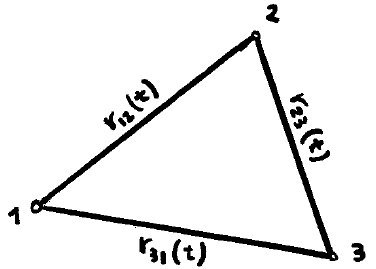
\includegraphics[scale=0.6]{Draw/lec4_8.png}
\end{center}
\caption{Hubble's law and the cosmological principle}
\label{fig:lec4_8}
\end{figure}

From the point of view of galaxy 1, galaxies 2 and 3 are moving away with velocities
\begin{equation}
\begin{split}
v_{12}(t)&=\frac{dr_{12}(t)}{dt}=\frac{da(t)}{dt}r_{12}(t_0)=\frac{\dot{a}}{a}r_{12}(t),\\
v_{31}(t)&=\frac{dr_{31}(t)}{dt}=\frac{da(t)}{dt}r_{31}(t_0)=\frac{\dot{a}}{a}r_{31}(t),\\
\end{split}
\end{equation}
where we introduced the notation
\begin{equation}
\dot{a}(t)\equiv \frac{da(t)}{dt}.
\end{equation}
Let us also define the {\it Hubble parameter}
\begin{equation}
H(t)\equiv \frac{\dot{a}(t)}{a(t)},
\end{equation}
which allows us to write the velocities $v_{12}$ and $v_{31}$ as
\begin{equation}
\begin{split}
v_{12}(t)&=H(t)r_{12}(t),\\
v_{31}(t)&=H(t)r_{31}(t).
\end{split}
\end{equation}
If we evaluate these formulas at $t=t_0$ (the present time), we find
\begin{equation}
\begin{split}
v_{12}(t_0)&=H_0 r_{12}(t_0),\\
v_{31}(t_0)&=H_0 r_{31}(t_0),
\end{split}
\end{equation}
where we have identified $H_0\equiv H(t_0)$, which says that the Hubble constant is simply the present value of the Hubble parameter. With this identification we see that these formulas reproduce Hubble's law for galaxy 1, since they state that galaxies 2 and 3 are receding from galaxy 1 at velocities proportional to their distances. But now we could repeat exactly the same analysis for galaxies 2 and 3, and find that Hubble's law also holds for them (and with the same proportionality constant $H_0$). We conclude from this argument that Hubble's law is consistent with an expansion of the universe that preserves homogeneity and isotropy. There is no violation of the cosmological principle here: just as we see other galaxies moving away from us, the inhabitants of any of these likewise see other galaxies receding from them.

Fig.\ \ref{fig:lec4_9} shows a more recent version of the graph used by Hubble to determine his expansion law. Each dot in the graph represents a galaxy, and one can clearly observe a linear relation between velocity and distance. An important observation, however, is that Hubble's law is only an approximate law, as can be seen from the fact that the dots in the graph do not follow a perfect straight line. This deviation from a ``perfect Hubble's law'' does not happen, of course, because the expansion of the universe is irregular (which would contradict the cosmological principle), but because of the {\it peculiar motion} of the galaxies. The peculiar motion is the motion that occurs due to the gravitational attraction of nearby galaxies, and has nothing to do with the expansion of the universe. For example, the Andromeda galaxy and the Milky Way are not moving away from each other, but they are actually moving closer due to the gravitational attraction that exists between them.
\begin{figure}[ht]
\begin{center}
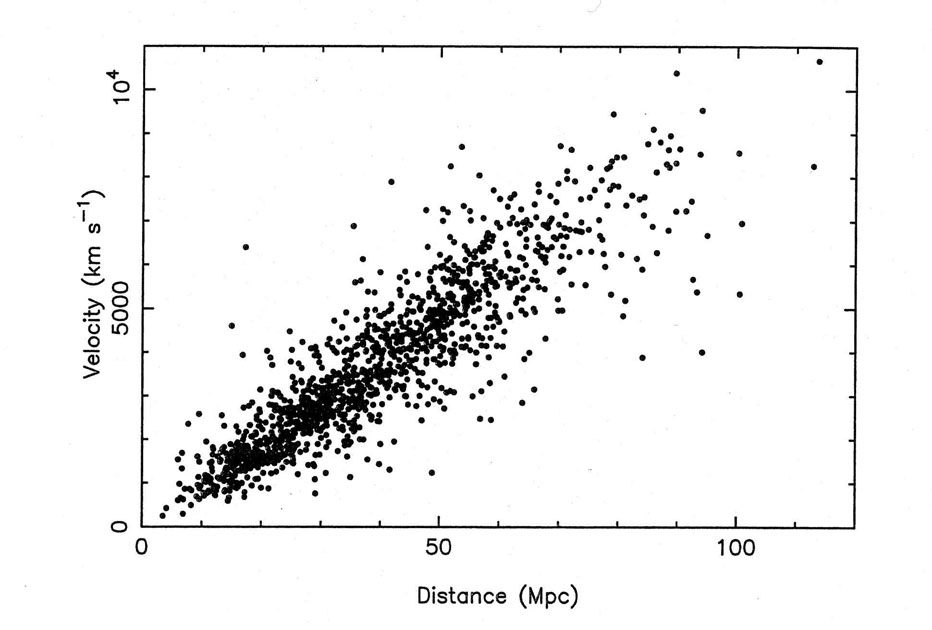
\includegraphics[scale=0.4]{Draw/lec4_9.png}
\end{center}
\caption{Hubble's law (Image credit: J. Imamura, University of Oregon)}
\label{fig:lec4_9}
\end{figure}

\subsubsection{The Big Bang}

If we watch the history of the universe running backward in time, we would see all the galaxies approaching each other. Then, if we assume that the universe has always been expanding, there must have been a time in the past when all particles were infinitely close to each other. In this picture, the universe was born from a state of infinite temperature and density, a state known as the Big Bang.

Consider two galaxies separated today by a distance $d$ and moving away from each other with a speed $v$. Then, by Hubble's law, $v=H_0 d$. Let us assume that the two galaxies have been always moving (relative to each other) with the same speed $v$. The time elapsed since the moment in which they were in contact is then
\begin{equation}
\begin{split}
t_0&=\frac{d}{v}=\frac{d}{H_0 d}=\frac{1}{H_0}\approx 14\times10^9~\mathrm{years}.
\end{split}
\end{equation}
We find that, under this assumption of constant expansion rate, the age of the universe would be roughly 14 billion years.\footnote{The constant $1/H_0$ is sometimes referred to as the Hubble time.} There are, however, two important caveats to this argument. First, $H(t)$ is a function of time, meaning that the expansion rate has not been always the same. How do we even know that the universe has always been expanding? Second, we have stressed above that the expansion of the universe is a large-scale effect; on small scales, the local interactions between bodies always dominate over the Hubble expansion. How do we know then that Hubble's law holds at the early times when the universe was very dense? To answer these questions we need to use GR. Specifically, we need to learn how to describe our universe by means of a metric, and then apply the Einstein equations to find how the scale factor $a(t)$ evolves in time. This will be the subject of the next lecture.